\paragraph{Desarrollo técnico}
Como intento de mejora a la anterior versión, la cual era de conversión directa, se trató de diseñar un receptor superheterodino. A su vez, se mantuvo el diseño del transmisor a varactores, pero se cambió la frecuencia de trabajo a una mayor, unos \SI{6}{\mega\hertz}. 
\paragraph{}
El diseño consistía en la recepci\'on de la señal mediante un filtro de entrada que posteriormente era introducida en un mezclador con un oscilador fijo. Después, se realizaba el tratamiento con la señal de frecuencia intermedia obtenida tras filtrar la señal de salida del mezclador. Posteriormente, esta señal atravesaba un amplificador de dos etapas y un rectificador con filtro paso bajo para ser demodulada. 
\paragraph{}
Se muestra un esquemático en la figura \ref{fig:crono_sch_receiver_varactor} del receptor sin la parte digital, la cual se explica en el apartado \ref{sec:crono_digital}. La figura \ref{fig:crono_sch_receiver_varactor}, consta de la parte de RF explicada a la derecha, y de la interfaz con la parte digital, un amplificador con realimentaci\'on positiva denominado \textit{Smith-trigger}.

\begin{figure}[h!]
    \centering
    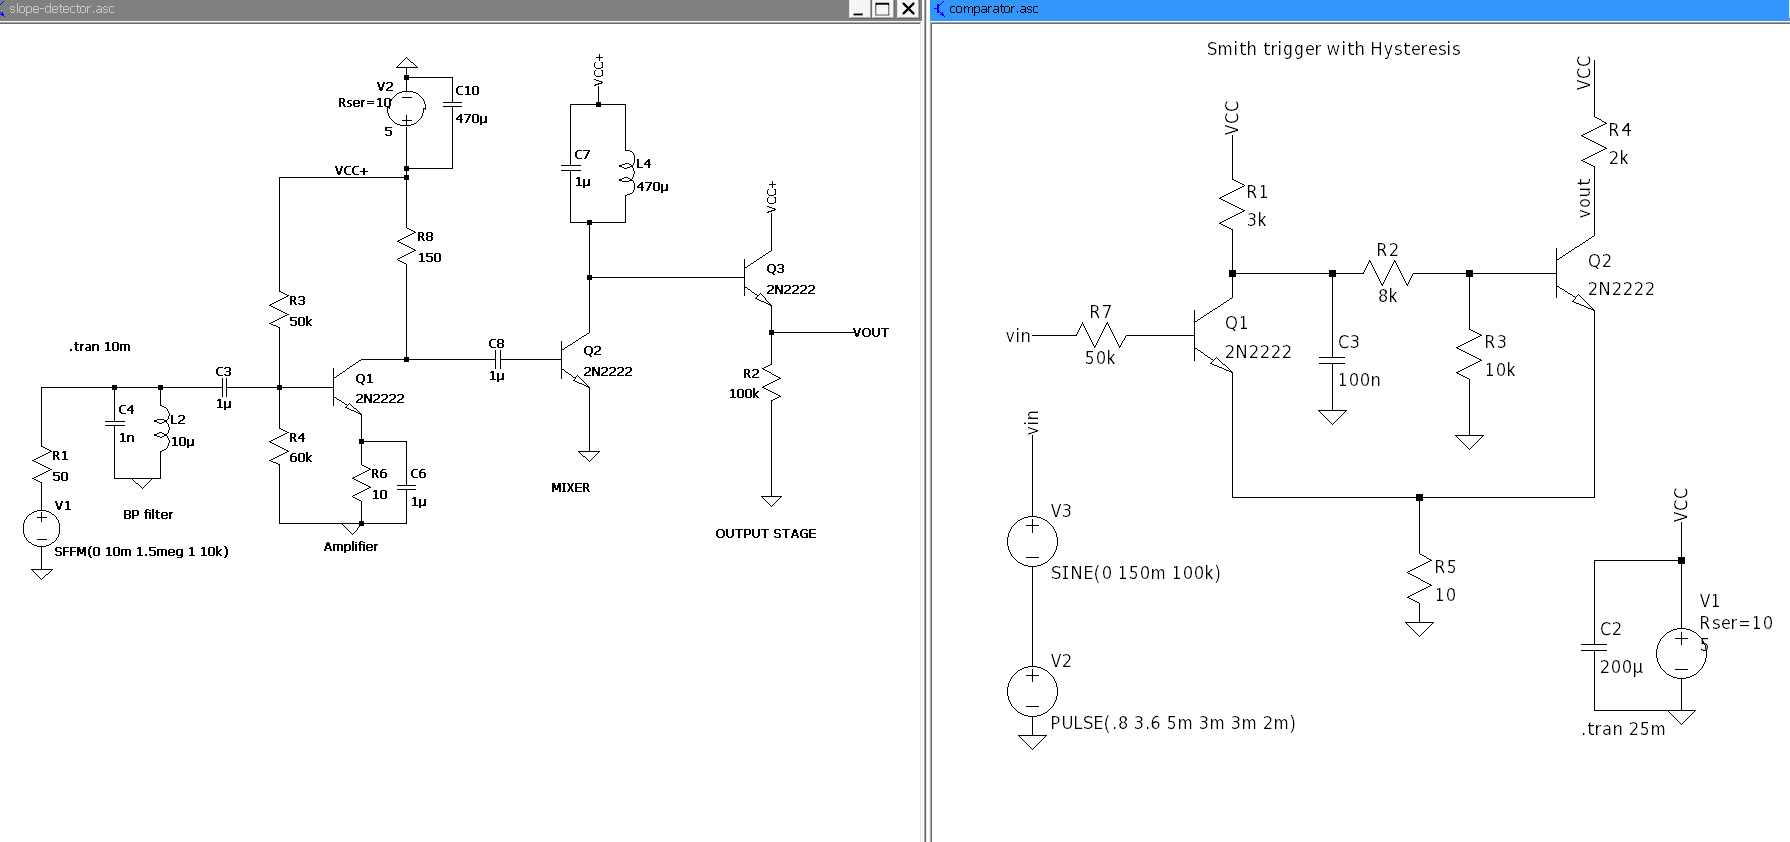
\includegraphics[scale=1, width=1\textwidth]{crono_sch_receiver_varactor}
    \caption{Modelo esquem\'atico del receptor superheterodino de FM}
    \label{fig:crono_sch_receiver_varactor}
\end{figure}

\paragraph{Motivos de reemplazo}
Este diseño funcionaba bien cuando se conectaba a la entrada un generador de frecuencias a la frecuencia de trabajo de muy baja potencia.
El problema surgía cuando se trataba de probar con el transmisor. 
El receptor no tenía buena selectividad y los amplificadores de frecuencia intermedia, los cuales no estaban correctamente diseñados, producían oscilaciones.
\paragraph{}
Gracias al mezclador, el circuito era capaz de detectar señales de muy baja potencia con muy buena selectividad, en caso de que la señal de entrada no fuera ruidosa. A pesar de todo, el mezclador era bastante sensible al ruido, ya que generaba bastantes armónicos, producidos por efectos de segundo orden. Esto provocaba que si a la señal de entrada se le añadían efectos de distorsión y ruido, el receptor estaba lejos de funcionar correctamente. 
%Esto explica el por qué al conectarlo con el generador, lo más cercano a un tono puro, funcionaba correctamente, sin embargo cuando se trataba de enlazar con la señal del transmisor la cosa cambiaba.
\paragraph{}
Por otro lado, en mi opinión, el diseño utilizaba demasiados componentes para unas prestaciones tan bajas. El diseño debía ser sencillo y funcional.
\paragraph{}
Debido a la complejidad, a cambio de ninguna clase de beneficio, se opt\'o por transicionar a un esquema de modulaci\'on AM.
